% ME3050 -  Dynamics Modeling and Controls - Tennessee Technological University
% Tristan Hill - Spring 2020 - Summer 2020 - Spring 2022
% Dynamics Modeling and Controls
% Lecture Module - Electrical Systems - Topic 4  - Mechatronics Applications

% Document settings

\documentclass[fleqn]{beamer}                  % for presentation ?
%\documentclass[handout]{beamer}  % for handout ?
 
%\usepackage{/home/thill/Documents/lectures/dmc_lectures/dmc_lectures}
\usepackage{/home/tntech.edu/thill/courses/dmc/dmc_lectures}

\newcommand{\MNUM}{2\hspace{2mm}} % Module number
\newcommand{\TNUM}{4\hspace{2mm}} % Topic number 
\newcommand{\moduletitle}{Electrical Systems} % Titles and Stuff
\newcommand{\topictitle}{Example: Brushed DC Motor} 

\newcommand{\sectiontitleI}{Brushed DC Motor}
\newcommand{\sectiontitleII}{Model Derivation}
\newcommand{\sectiontitleIII}{State Space Form}
\newcommand{\sectiontitleIV}{Transfer Functions}
\newcommand{\sectiontitleV}{Simulated Response}

\author{ME3050 - Dynamic Modeling and Controls}
\title{Lecture Module - \moduletitle}
\date{Mechanical Engineering\vspc Tennessee Technological University}

\lstset{language=MATLAB,basicstyle=\ttfamily\small,showstringspaces=false}

\makeatletter
\renewcommand*\env@matrix[1][\arraystretch]{%
  \edef\arraystretch{#1}%
  \hskip -\arraycolsep
  \let\@ifnextchar\new@ifnextchar
  \array{*\c@MaxMatrixCols c}}
\makeatother
\begin{document}
	
	\lstset{language=MATLAB,basicstyle=\ttfamily\small,showstringspaces=false}
	
	\frame{\titlepage \center\begin{framed}\Large \textbf{Topic \TNUM - \topictitle}\end{framed} \vspace{5mm}}
	
	% Section 0 - Outline
\frame{
	
	\large \textbf{\moduletitle} \vspace{3mm}\\
	
	\begin{itemize}
	
		\item \hyperlink{sectionI}{\sectiontitleI} \vspc % Section I
		\item \hyperlink{sectionII}{\sectiontitleII} \vspc % Section II
		\item \hyperlink{sectionIII}{\sectiontitleIII} \vspc %Section III
		\item \hyperlink{sectionIV}{\sectiontitleIV} \vspc %Section IV	
		\item \hyperlink{sectionV}{\sectiontitleV} \vspc %Section V
	
	\end{itemize}

}

	% Section I
	\section{\sectiontitleI}

	% Section I - Frame I
	\begin{frame}[label=sectionII,containsverbatim] \small
        \frametitle{\sectiontitleII}
		Armature Controlled Brushed DC Motor \vspc

		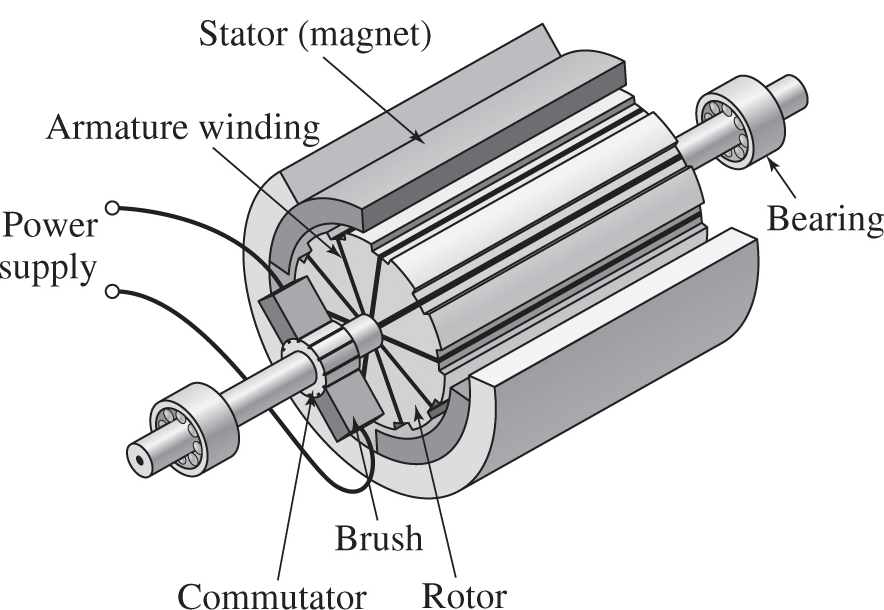
\includegraphics[scale=.85]{paL40056_06_05_03_cropped.png}

		\btVFill
		\tiny{Image: System Dynamics, Palm, 4$^{th}$, Pg. 376-378}
		
	\end{frame}

	% Section I - Frame II
	\begin{frame}[label=sectionI] \small
		\frametitle{\sectiontitleI}

		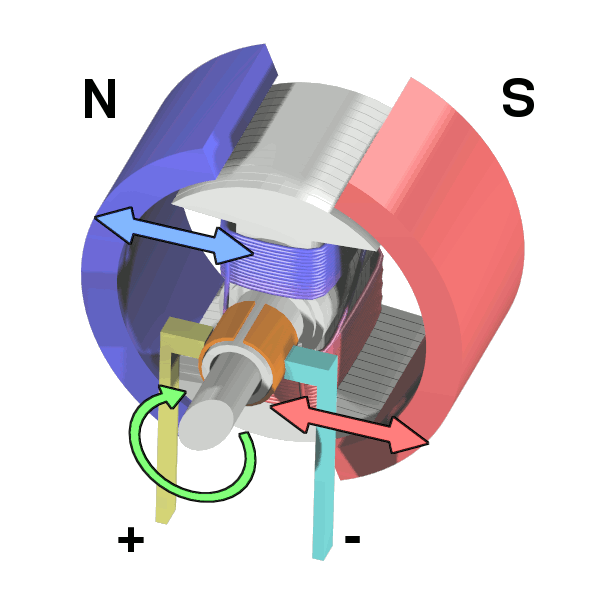
\includegraphics[scale=.25]{Electric_motor_cycle_2.png}

		\href{https://en.wikipedia.org/wiki/DC_motor}{Animation on Web} 

		\btVFill
		\tiny{source: \href{https://en.wikipedia.org/wiki/DC_motor}{wikipedia}}
	\end{frame}	

    % Section II
    \section{\sectiontitleII}

	% Section II - Frame I
	\begin{frame}[label=sectionII,containsverbatim] \small
        \frametitle{\sectiontitleII}
		Armature Controlled Brushed DC Motor \vspc

		\begin{multicols}{2}

		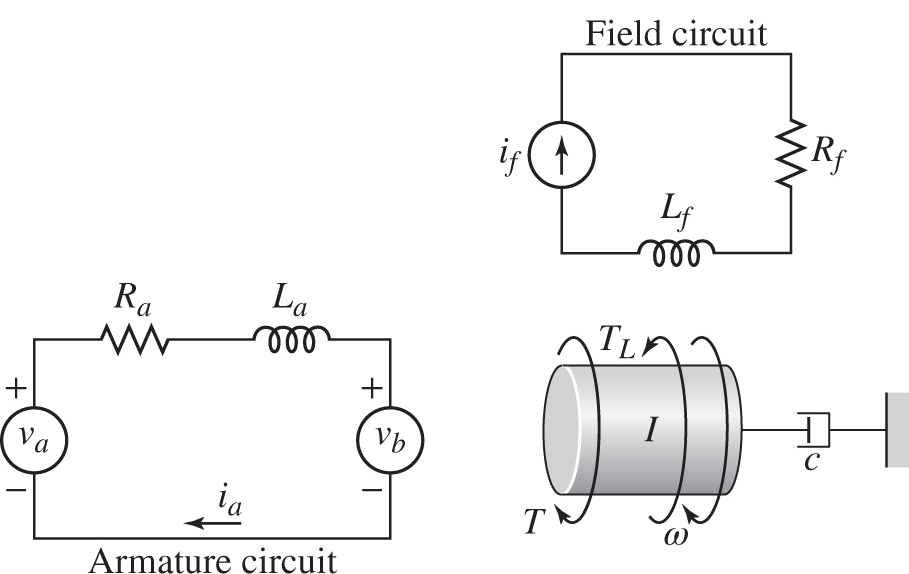
\includegraphics[scale=.70]{paL40056_06_05_04_cropped.png}\vspace{5mm}\\

		\small
		$v_a$ : armature voltage (input)\vspc
        $R_a$ : armature resistance

        Torque on armature
        \[T=\left(nBLi_a \right)r=\left(nBLr\right)i_a=K_Ti_a \] 
        Back EMF (electromotive force) voltage
        \[v_b=nBLv=\left(nBLr\right)\omega=K_b\omega \]	

        \end{multicols}

		\btVFill
		\tiny{Image: System Dynamics, Palm, 4$^{th}$, Pg. 376-378}
		
	\end{frame}

	% Section II - Frame II
	\begin{frame}[label=sectionII,containsverbatim] \small
        \frametitle{\sectiontitleII}
		Armature Controlled Brushed DC Motor \vspc

		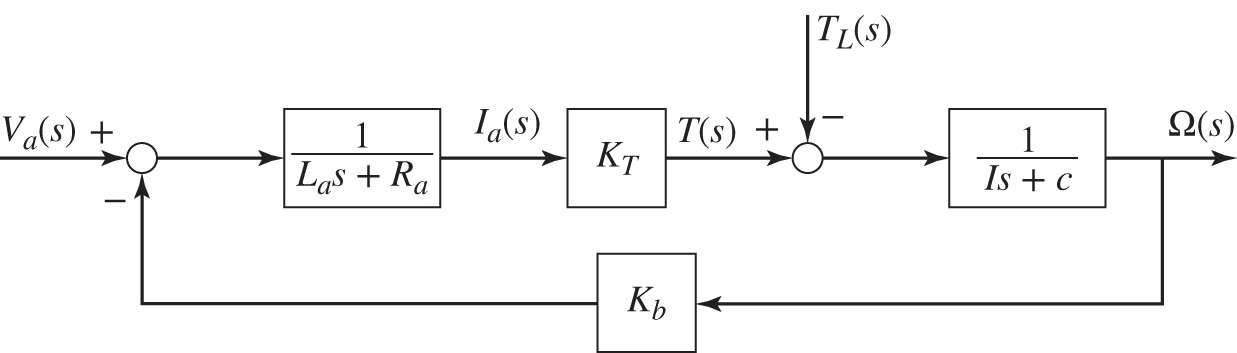
\includegraphics[scale=.65]{paL40056_06_05_05_cropped.png}

        Kirchoff's Voltage Law 
        \[ v_a-R_ai_a-L_a\frac{di_a}{dt}-K_b\omega=0 \] 

        Newtons's Second Law  
        \[ I\frac{d\omega}{dt}=T-c\omega-T_L=K_Ti_a-c\omega-T_L \]	

		\btVFill
		\tiny{Image: System Dynamics, Palm, 4$^{th}$, Pg. 376-378}
		
	\end{frame}	


	% Section III
	\section{\sectiontitleIII}

	% Section III - Frame III
	\begin{frame} \small
		\frametitle{\sectiontitleIII}

		State-Variable (State-Space) form
		\[\renewcommand*{\arraystretch}{1.5}
		  \frac{di_a}{dt}=\dot{x}_1=\frac{1}{L_a}\left( v_a -R_ai_a-K_b\omega\right)
		  = \begin{bmatrix} -\frac{R_a}{L_a} & -\frac{K_b}{L_a} \end{bmatrix}
		  \begin{bmatrix} x_1 \\ x_2 \end{bmatrix}
		  +\begin{bmatrix} \frac{1}{L_a} & 0 \end{bmatrix}
		  \begin{bmatrix} v_a \\ T_L \end{bmatrix}
		\]
		\[
		  \frac{d\omega}{dt}=\dot{x}_2=\frac{1}{I}\left( K_Ti_a-c\omega-T_L\right)	
		  = \begin{bmatrix} -\frac{K_T}{I} & -\frac{c}{I} \end{bmatrix}
		  \begin{bmatrix} x_1 \\ x_2 \end{bmatrix}
		  +\begin{bmatrix} 0 & -\frac{1}{I} \end{bmatrix}
		  \begin{bmatrix} v_a \\ T_L \end{bmatrix}
		\]

		Write the state equation in matrix form with states $x_1=i_a$, and $x_2=\omega$
		\[
		  \begin{bmatrix}\dot{x}_1 \\ \dot{x}_2\end{bmatrix} 
		  =\begin{bmatrix}[1.5] -\frac{R_a}{L_a} & -\frac{K_b}{L_a} \\ \frac{K_T}{I} & -\frac{c}{I}\end{bmatrix}
		  \begin{bmatrix} x_1 \\ x_2\end{bmatrix}
		  +\begin{bmatrix}[1.5] \frac{1}{L_a} & 0 \\ 0 & -\frac{1}{I}\end{bmatrix}
		  \begin{bmatrix}v_a \\T_L \end{bmatrix}
        \]

	\end{frame}	

% Section IV
\section{\sectiontitleIV}

	% Section IV - Frame I
	\begin{frame}[label=sectionIV] \small
		\frametitle{\sectiontitleIV}
		The input-output relationships can be represented by the following transfer functions.\vspc

		Armature Current to Armature Voltage
		\[\frac{I_a\left(s\right)}{V_a\left(s\right)}=\frac{Is+c}{L_aIs^2+\left(R_aI+cL_a\right)s+cR_a+K_bK_T}\]
		
		Armature Current to External Load
		\[\frac{I_a\left(s\right)}{T_L\left(s\right)}=\frac{K_b}{L_aIs^2+\left(R_aI+cL_a\right)s+cR_a+K_bK_T}\]

	\end{frame}	

	% Section IV - Frame II
	\begin{frame}[label=sectionIV] \small
		\frametitle{\sectiontitleIV}

		Armature Angular Velocity to Armature Voltage
		\[\frac{\Omega\left(s\right)}{V_a\left(s\right)}=\frac{K_T}{L_aIs^2+\left(R_aI+cL_a\right)s+cR_a+K_bK_T}\]
		
		Armature Angular Velocity to External Load
		\[\frac{\Omega\left(s\right)}{T_L\left(s\right)}=\frac{L_as+R_a}{L_aIs^2+\left(R_aI+cL_a\right)s+cR_a+K_bK_T}\]
		
	\end{frame}	

	% Section IV - Frame II
	\begin{frame}[label=sectionIV] \small
		\frametitle{\sectiontitleIV}

		\textbf{Final Value Theorem:} 
		To find the value of a function $x(t)$ as $t\rightarrow \infty$  

		\[x\left(\infty\right)=\lim_{x\to\infty} f(x) = \lim_{s\to 0} sX\left(s\right)\]

		Use final value theorem to find steady state value to step input on $V_a$, $T_L$
		\[i_a=\frac{cV_a + K_bT_L}{cR_a+K_bK_T}\]

		\[\omega=\frac{K_TV_a-R_aT_L}{cR_a+K_bK_T}\]

	\end{frame}

% Section V
\section{\sectiontitleV}

	% Section V - Frame I
	\begin{frame}[containsverbatim,label=sectionV] \small
		\frametitle{\sectiontitleV}

		The following MATLAB code defines a state space system object and simulates the system response to various inputs.
		
		\begin{lstlisting}
% DC Motor Example (System Dynamics 4th ed., Palm, Pg 376-378)  
clear; close all; clc

% define system parameters
KT=0.05;  % (N*m/A)
Kb=KT;    % (N*m/A)
c=10e-4;  % (N*m*s/rad)   
Ra=0.5;   % (Ohm)
La=2e-3;  % (H)
I=9e-5;   % (kg*m^2)
		\end{lstlisting}
\end{frame}	

% Section V - Frame II
	\begin{frame}[containsverbatim,label=sectionV] \small
		\frametitle{\sectiontitleV}
		\begin{lstlisting}
% define components of the state equation
A=[-Ra/La -Kb/La
   KT/I -c/I];
% B matrix is 2x2 because u vector is 2x1
B=[1/La 0 
   0 -1/I];

% use first two states as outputs
C=[1 0
   0 1];
% the D matrix shape of B matrix 
D=[0 0
   0 0];
		\end{lstlisting}
	\end{frame}

% Section V - Frame III
	\begin{frame}[containsverbatim,label=sectionV] \small
		\frametitle{\sectiontitleV}
		\begin{lstlisting}
% calculate the steady state step response
Va=12;
TL=0;
ia_ss=(c*Va+Kb*TL)/(c*Ra+Kb*KT)

% create a state space model object
sys1=ss(A,B,C,D);

% simulate a step response 
figure(1)
time=0:0.001:1;
opts=stepDataOptions('StepAmplitude',Va);
step(sys1,time,opts); grid on
		\end{lstlisting}

	\end{frame}	

% Section V - Frame III
	\begin{frame}[containsverbatim,label=sectionV] \small
		\frametitle{\sectiontitleV}
		
		\begin{multicols}{2}

		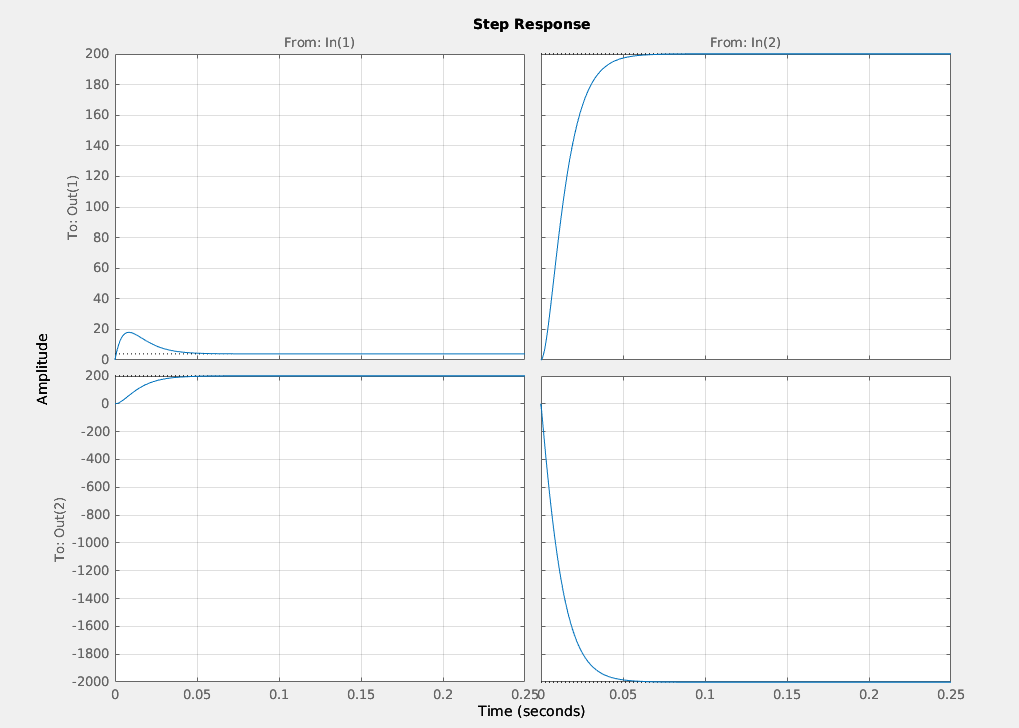
\includegraphics[scale=0.25]{dc_motor_state_space_figure1.png}	

		\begin{lstlisting}
ia_ss =

    4.0000

w_ss =

   200
		\end{lstlisting}

		\end{multicols}

	\end{frame}

\end{document}
